\documentclass[a4paper]{article}

\usepackage[margin=1in]{geometry}
\usepackage{amsmath}
\usepackage{amssymb}
\usepackage{graphicx}
\usepackage{float}
\usepackage{hyperref}
\usepackage[outputdir=out]{minted}
\usepackage{subcaption}
\usepackage{amsfonts}
\usepackage{pdfpages}
\usepackage[justification=centering]{caption}
\usepackage{algpseudocode}

\def\sectionautorefname{Section}
\def\subsectionautorefname{Section}
\def\subsubsectionautorefname{Section}
\def\figureautorefname{Figure}
\def\tableautorefname{Table}
\def\equationautorefname{Equation}


\begin{document}

    \title{Logistic Classification}
    \author{3F8: Inference Coursework \\ Theo Brown \\ Selwyn College, University of Cambridge}
    \date{\today}
    \maketitle

    \begin{abstract}
        The method of logistic regression using gradient ascent optimisation is presented as a means of training a
        linear classifier. The linear classifier is trained on a test data set, and shown to perform poorly. A set of
        non-linear basis functions are introduced, which can be applied to the input data to enable the logistic
        regression model to fit to non-linear data sets. The classifier using basis functions is shown to perform well
        on the data set, after tuning of the basis function parameters.
    \end{abstract}

    \section{Introduction}\label{sec:introduction}
    Classification is the task of grouping data points according to their shared features, and assigning each group
    a label. For a human with a small dataset, this is a trivial task, but it is much more difficult and slow with very
    large or complex data sets. Consequently, the development of good machine classifiers is an important area in
    statistical learning. Trained classifiers can be used as predictive tools to identify the most probable class that a
    new input will belong to, which could, for example, be useful in a medical setting, such as identifying the most
    at-risk patients.

    A key tool in classification is the ability to classify non-linear datasets, where the boundary between classes
    is not a straight line. This report demonstrates the failure of a linear classifier on a non-linear dataset, and
    explores the use of a set of non-linear basis functions (in this case, radial functions) applied to the inputs before
    classifying to allow the discovery of non-linear decision boundaries.

    \section{Derivation of the gradient of the log-likelihood}\label{sec:gradient-derivation}
    Define the n-th input vector as $\textbf{x}_n$, and let the augmented input vector
    $\tilde{\textbf{x}}_n = \left[1, \textbf{x}_n^T \right]^T$.
    The set of augmented input vectors are assembled as the columns of matrix
    $\tilde{\textbf{X}} = [\tilde{\textbf{x}}_1, \dots, \tilde{\textbf{x}}_N]$.
    Define $\sigma(x) = \frac{1}{1 + e^{-x}}$.
    The class labels, $\textbf{y}$, are modelled as being independent and identically generated from a Bernoulli
    distribution, with $p (y_n = 1 | \tilde{\textbf{x}}_n ) = \sigma (\textbf{w}^T\tilde{\textbf{x}}_n)$ and
    $p (y_n = 0 | \tilde{\textbf{x}}_n ) = 1 - \sigma (\textbf{w}^T\tilde{\textbf{x}}_n) = \sigma (-\textbf{w}^T\tilde{\textbf{x}}_n)$,
    where $\textbf{w}$ is a vector of model weights.
    The log-likelihood of \textbf{w} is therefore:
    \begin{align*}
        \mathcal{L}(w) = \log p(y|\tilde{\textbf{X}}, \textbf{w})
        &= \log \prod_{n=1}^{N} \sigma( \textbf{w}^T \tilde{\textbf{x}}_n)^{y_n}
        \sigma (-\textbf{w}^T \tilde{\textbf{x}}_n)^{1-y_n} \\
        &= \sum_{n=1}^{N} y_n \log\sigma( \textbf{w}^T \tilde{\textbf{x}}_n) + (1-y_n) \log\sigma(-w^T \tilde{\textbf{x}}_n)
    \end{align*}
    The derivative of the log-likelihood is calculated using the identities $\frac{d\sigma(x)}{dx} = \sigma(x)\sigma(-x)$
    and $\frac{d\log(x)}{dx} = \frac{1}{x}$. Applying the chain rule:
    \begin{align*}
        \frac{\partial \mathcal{L}}{\partial w}
        &= \sum_{n=1}^{N} y_n \sigma(-\textbf{w}^T \tilde{\textbf{x}}_n) \tilde{\textbf{x}}_n - (1-y_n) \sigma(\textbf{w}^T \tilde{\textbf{x}}_n)  \tilde{\textbf{x}}_n \\
        &= \sum_{n=1}^{N} \left(y_n - \sigma(\textbf{w}^T \tilde{\textbf{x}}_n) \right)  \tilde{\textbf{x}}_n \\
        &= \tilde{\textbf{X}} (\textbf{y} - \sigma(\tilde{\textbf{X}}^T \textbf{w}))
    \end{align*}

    \section{Gradient ascent algorithm}\label{sec:gradient-ascent-algorithm}
    To find the parameter $\textbf{w}$ that maximises the log-likelihood, a gradient ascent algorithm is used. Define
    $\tilde{\textbf{X}}$ and y as in \autoref{sec:gradient-derivation}, then let n be the number of iterations to run the
    algorithm for and r be the learning rate. The algorithm is defined as follows:

    \begin{algorithmic}
        \Procedure{GradientAscent}{$\tilde{\textbf{X}}$, $\textbf{y}$, n, r}
            \State $\textbf{w} \gets [0 \dots 0]^T$ \Comment{Initialise the weights}
            \For{$i\gets 1, n$}
                \State $\textbf{d} \gets \tilde{\textbf{X}} (\textbf{y} - \sigma(\tilde{\textbf{X}}^T \textbf{w})))$ \Comment{Calculate the gradient}
                \State $\textbf{w} \gets \textbf{w} + r\textbf{d} $ \Comment{Move along the gradient, scaled by learning rate}
            \EndFor
        \EndProcedure
    \end{algorithmic}

    Note that the weights do not necessarily need to be initialised as zeros - they could have been selected randomly, or
    initialised as ones, for example. Provided the number of iterations is large enough and the algorithm does not get
    stuck in a local maximum, the effect of the initial values should be negligible.

    The learning rate, n, is chosen empirically. Starting with a value chosen such the algorithm shows signs
    of convergence, the learning rate is increased until the algorithm begins to oscillate. The rate is then decreased
    slightly so that the oscillation is avoided. Using this method, a fast rate of convergence is ensured and divergence
    avoided.

    In Python\footnote{The Python 3.5+ matrix multiplication operator $@$ provides an easy method of vectorising the
    operations}, the gradient ascent algorithm can be implemented as follows, noting the necessary alterations from
    column to row vectors:

    \begin{minted}{python}
        import numpy as np

        def logistic(x):
            return 1 / (1 + np.exp(-x))

        def gradient_ascent(X, y,
                            number_iterations, learning_rate):
            # Prepend a column of ones to the input data (X)
            X1 = np.column_stack((np.ones(X.shape[0]), X))
            # Initialise the weights
            w = np.ones(X1.shape[1])

            for i in range(number_iterations):
                # Calculate the gradient
                dL = (y - logistic(X1 @ w)) @ X1
                # Move in the direction of the gradient,
                # scaled by learning rate
                w += learning_rate * dL
            return w
    \end{minted}

    \section{Data visualisation}\label{sec:data-visualisation}
    The data is visualised in the two-dimensional input space in \autoref{fig:data}. From the plot it is clear that a
    linear classifier will perform badly on the data, as the classes are not linearly separable: there is no straight
    boundary that successfully distinguishes between red and blue data points.

    \section{Linear classifier training}\label{sec:linear-training}
    The data was split into a training set of 800 points and a test set of 200 points, and the gradient descent
    algorithm with a learning rate of 0.001 was applied to find the weights for the linear classifier. The mean
    log-likelihood (where the mean is taken across all of the weights) is plotted in \autoref{fig:linear_log_likelihood} for
    the training and test datasets at each iteration.

    \begin{figure}
        \begin{minipage}{0.32\textwidth}
            \centering
            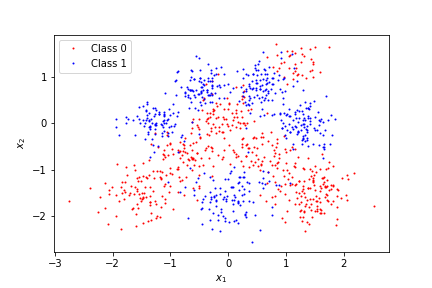
\includegraphics[width=\textwidth]{plots/ml_logistic_regression/data}
            \captionof{figure}{Plot of the two-dimensional input features (1000 datapoints, 2 classes)}
            \label{fig:data}
        \end{minipage}%
        \begin{minipage}{0.32\textwidth}
            \centering
            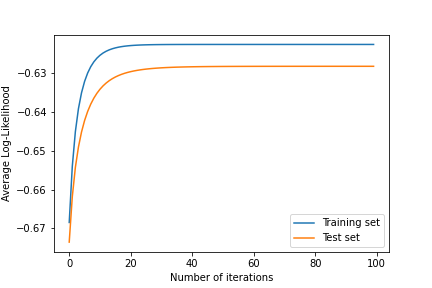
\includegraphics[width=\textwidth]{plots/ml_logistic_regression/log_likelihood}
            \captionof{figure}{Plot of the mean log-likelihood of the weights for the test and training data, over the
            course of model training}
            \label{fig:linear_log_likelihood}
        \end{minipage}%
        \begin{minipage}{0.32\textwidth}
            \centering
            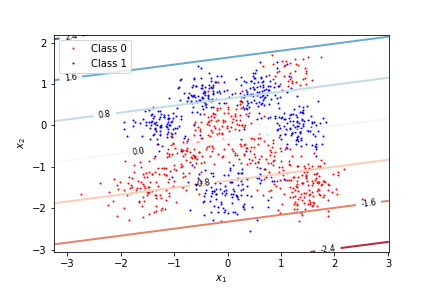
\includegraphics[width=\textwidth]{plots/ml_logistic_regression/predictive_distribution_linear}
            \captionof{figure}{Model predictive distribution overlaid on input datapoints coloured by class}
            \label{fig:linear_predictive_distribution}
        \end{minipage}
    \end{figure}

    \autoref{fig:linear_log_likelihood} shows that a plateau is reached for the log-likelihood of the parameters in both the
    training and test sets, after which no further improvements can be made. This suggests an optimum has been found for
    this model. After training there remains a difference between the performance on the test and training sets, but not
    at a significant level (see \autoref{sec:linear-performance}).

    \section{Linear classifier performance}\label{sec:linear-performance}
    The predictive distribution of the model is shown in \autoref{fig:linear_predictive_distribution}. It is clear that
    this model fails to accurately classify the two classes. It identifies that the general principle that more of the
    points with $x_2 < 0$ are class 1 and more of the points with $x_2 > 0$ values are class 2, but it is apparent to
    the human eye that this is overly simplified and fails to identify the `islands' where one class appears surrounded
    by the other.

    The mean log-likelihood of the trained model evaluated on the training and test sets is shown in
    \autoref{tab:performance_metrics_linear}. It shows a difference of about 2\% between the training and test data, which is
    sufficiently small to suggest that overfitting has been avoided. As expected, the performance is marginally better
    for the training set, as this was the data that the model was fit to. The main issue here is clearly not overfitting,
    instead it is apparent that the model is insufficient.

    To find the predicted class label for a point $\boldsymbol{x}_n$, a hard threshold is applied to the predicted class
    probabilities:
    \begin{align*}
        \hat{y}_n = \begin{cases}
                        0 & \sigma(\tilde{\boldsymbol{x}}_n^T \boldsymbol{w}) \leq 0.5 \\
                        1 & \sigma(\tilde{\boldsymbol{x}}_n^T \boldsymbol{w}) > 0.5
                    \end{cases}
    \end{align*}

    Using the predicted class labels, the confusion matrix for the test data is found
    (\autoref{tab:performance_metrics_linear}). The confusion matrix is a good method of assessing the classifier's
    performance, as it shows the fraction of correct and incorrect classifications for each class.

    \autoref{tab:performance_metrics_linear} shows that the linear classifier successfully identifies class 0 about
    70\% of the time. Comparing with \autoref{fig:linear_predictive_distribution}, we can see that the decision boundary
    (shown as a contour of value 0.0) correctly separates roughly four out of six visually identifiable clusters of
    class 0, and fails to account for two. Similarly, the classifier identifies class 1 69\% of the time, and the
    decision boundary separates approximately three and a half out of five visually identifiable class 1 clusters.

    \begin{table}[h]
        \centering
        \begin{tabular}{c|c}
            \textbf{Performance metric} & \textbf{Value} \\
            \hline
            Mean log-likelihood, training data & -0.623 \\
            Mean log-likelihood, test data & -0.628 \\
            $\begin{pmatrix}
                 P(\hat{y}=0 | y=0) & P(\hat{y}=1 | y=0) \\
                 P(\hat{y}=0 | y=1) & P(\hat{y}=1 | y=1) \\
            \end{pmatrix}$ &
            $\begin{pmatrix}
                0.707 & 0.293 \\
                0.306 & 0.694 \\
            \end{pmatrix}$ \\
        \end{tabular}
        \caption{Performance metrics for the linear classifier}
        \label{tab:performance_metrics_linear}
    \end{table}

    It's clear that, as expected, the linear classifier does not provide a particularly useful result for this dataset.
    A new method is presented in the next section, which uses a set of non-linear basis functions to allow the classifier to
    identify non-linear class boundaries.

    \section{Non-linear classifier definition and training}\label{sec:nonlinear-classifier}
    In order to identify non-linear class boundaries, the inputs can be expanded through a set of non-linear basis functions.
    Then the same logistic regression approach can be used to create the classifier.
    First, define a radial basis function (RBF) of the distance between two datapoints of dimension D, with width parameter l, as:
    \begin{align*}
        r(\textbf{x}_n, \textbf{x}_m, l) = \exp \left(-\frac{1}{2l^2} \sum_{d=1}^D (\textbf{x}_{n, d} - \textbf{x}_{m, d})^2 \right)
    \end{align*}
    Then define a new set of N augmented input vectors $\tilde{\textbf{x}}_n = [1, r(\textbf{x}_n, \textbf{x}_1, l), \dots, r(\textbf{x}_n, \textbf{x}_N, l)]^T$.
    The augmented input vectors are assembled into a matrix, as before, and the data split into test and training data sets.
    The gradient descent algorithm from \autoref{sec:gradient-ascent-algorithm} was applied to find the model weights,
    for RBFs with $l$ = 0.01, 0.1, and 1.
    The learning rate was set empirically for each value of the parameter $l$.

    \section{Non-linear classifier performance}\label{sec:nonlinear-performance}

    \autoref{tab:performance_metrics_nonlinear} shows the performance metrics for the classifier with different basis
    function widths.

    It is apparent that when $l = 0.01$, the model is drastically overfit to the training data, achieving
    a very small log-likelihood for the training data but scoring very poorly for the test data. \autoref{fig:nonlinear_predictive_distribution_0.01}
    shows decision boundaries that are effectively surrounding each individual training data point, which
    illustrates the overfitting.
    From the confusion matrix it is evident that this classifier is strongly biased towards class 0, successfully identifying class 0 95\% of the time
    but also falsely classifying 85\% of class 1 as class 0.

    \begin{figure}[h!]
        \begin{subfigure}{0.32\textwidth}
            \centering
            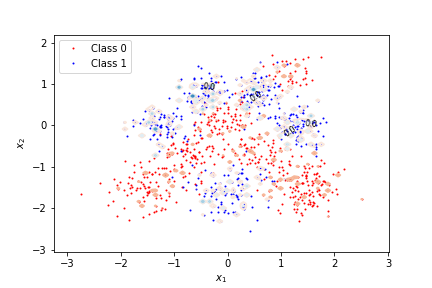
\includegraphics[width=\textwidth]{plots/ml_logistic_regression/predictive_distribution_nonlinear_w=0.01}
            \caption{$l$=0.01}
            \label{fig:nonlinear_predictive_distribution_0.01}
        \end{subfigure}
        \begin{subfigure}{0.32\textwidth}
            \centering
            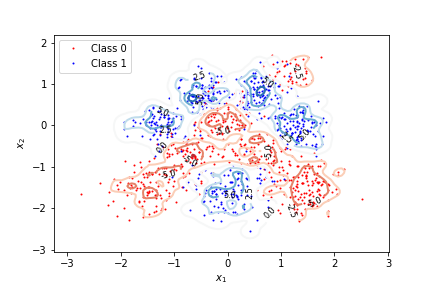
\includegraphics[width=\textwidth]{plots/ml_logistic_regression/predictive_distribution_nonlinear_w=0.1}
            \caption{$l$=0.1}
            \label{fig:nonlinear_predictive_distribution_0.1}
        \end{subfigure}
        \begin{subfigure}{0.32\textwidth}
            \centering
            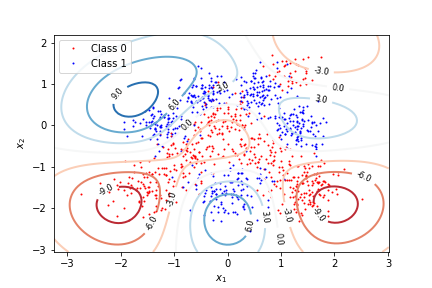
\includegraphics[width=\textwidth]{plots/ml_logistic_regression/predictive_distribution_nonlinear_w=1}
            \caption{$l$=1}
            \label{fig:nonlinear_predictive_distribution_1}
        \end{subfigure}
        \caption{Non-linear classifier predictive distributions}
        \label{fig:nonlinear_predictive_distributions}
    \end{figure}

    \begin{table}[h!]
        \centering
        \begin{tabular}{c|c|c|c}
            \textbf{Performance metric} & \textbf{$l$ = 0.01} & \textbf{$l$ = 0.1} & \textbf{$l$ = 1}\\
            \hline
            Mean log-likelihood, training data & -0.193 & -0.110 & -0.198 \\
            Mean log-likelihood, test data & -0.677 & -0.299 & -0.272 \\
            $\begin{pmatrix}
                 P(\hat{y}=0 | y=0) & P(\hat{y}=1 | y=0) \\
                 P(\hat{y}=0 | y=1) & P(\hat{y}=1 | y=1) \\
            \end{pmatrix}$ &
            $\begin{pmatrix}
                0.957 & 0.043 \\
                0.852 & 0.148 \\
            \end{pmatrix}$ &
            $\begin{pmatrix}
                0.902 & 0.098 \\
                0.139 & 0.861 \\
            \end{pmatrix}$ &
            $\begin{pmatrix}
                0.902 & 0.098 \\
                0.102 & 0.898 \\
            \end{pmatrix}$ \\
        \end{tabular}
        \caption{Performance metrics for the linear classifier}
        \label{tab:performance_metrics_nonlinear}
    \end{table}

    Increasing the width of the basis function to $l = 0.1$ drastically improves the classifier's performance,
    returning smaller log-likelihoods (suggesting it is more optimal) and improving the reliability of classifying class
    1. In particular note that the difference in performance on the training set and test set has been reduced, implying
    that the classifier is less overfitted. \autoref{fig:nonlinear_predictive_distribution_0.1} still exhibits a similar
    property to \autoref{fig:nonlinear_predictive_distribution_0.01}, where the decision regions are very close to the data,
    hence this classifier would perform poorly in labelling new points that lay further from the main clusters of each class.

    Further increasing the width continues to improve the classifier's performance, narrowing the gap between
    performance on the test and training sets, and improving the percentage of correct classifications for class 1.
    \autoref{fig:nonlinear_predictive_distribution_1} shows that the decision regions now extend beyond the data points,
    and nicely divide the $(x_1, x_2)$ plane. This is more the behaviour that we expect for a classifier,
    although perhaps in this example it is extrapolating too far from the data.

    It is likely that further optimisation of the width parameter $l$ would be fruitful in improving the
    classifier's performance.

    The best performance of the non-linear classifier is a dramatic improvement over the linear classifier, achieving 90\%
    success rate in identifying points of each class compared to the linear classifier's 70\%. The log-likelihood has also
    been reduced, suggesting that this model is a better fit to the data.

    \section{Conclusions}
    The method presented here is a powerful tool for developing classifiers. It is straightforward to find the
    model weights for the logistic model, using well-known and easily optimised gradient ascent algorithms. The equations
    are simple to vectorise, which makes them inexpensive to calculate on a computer.

    The importance of understanding the data before attempting to create a model is demonstrated by the failure
    of the linear classifier. Before embarking on developing the classifier, the expected shape of the data must be
    appreciated - is the data linearly separable? If not, then additional steps must be taken.

    Expanding the inputs through basis functions, such as the radial function presented here, unlocks the potential
    to classify non-linear data sets. A non-linear classifier using this method can be very successful, at minimal
    additional cost.

    The parameters of the gradient ascent algorithm and the basis functions must be chosen carefully
    to ensure convergence on an appropriate, non-overfitted model.
\end{document}